%!TEX root = ../chapter07.tex 
%----------------------------------------------------------------------------------------
%	
%----------------------------------------------------------------------------------------
%----------------------------------------------------------------------------------------
%	 
%----------------------------------------------------------------------------------------
%----------------------------------------------------------------------------------------
%	 
%----------------------------------------------------------------------------------------

\newpage  
\section{Exercices de mise en équation}
\begin{example} Retrouver l'écriture en fraction irréductible du rationnel dont l'écriture décimale périodique infinie est connue.
	
	\noindent \parbox{0.25\linewidth}{	
		$\begin{WithArrows}
			x&=0,\underline{7} \\ 
			x&=\numprint{0.777}\ldots \\
			&  \rule{0pt}{1.3em} \\
			&   \rule{0pt}{1.3em}  \\
			&   \rule{0pt}{1.3em} 
		\end{WithArrows}$ 	
	}\hfill \parbox{0.25\linewidth}{	
		$\begin{WithArrows}
			y&=0,\underline{37} \\ 
			y&=\numprint{0.373737}\ldots \\
			&  \rule{0pt}{1.3em} \\
			&   \rule{0pt}{1.3em}  \\
			&   \rule{0pt}{1.3em} 
		\end{WithArrows}$ 	
	}\hfill \parbox{0.40\linewidth}{	
		$\begin{WithArrows}
			z&=1,4\underline{37} \\ 
			z&=\numprint{1.4373737}\ldots \\
			&  \rule{0pt}{1.3em} \\
			&   \rule{0pt}{1.3em}  \\
			&   \rule{0pt}{1.3em} 
		\end{WithArrows}$ 	
	} 
\end{example}
\begin{exercise} \label{chapter07:exercice:miseenequation00} Même consignes : 
	\begin{multicols}{3}
		\begin{enumerate}[label={$\alph*=$}, leftmargin=*]
			\item $0,\underline{5}=\numprint{0.555}\ldots$  
			\item $0,\underline{14}=\numprint{0.141414}\ldots$ 
			\item $0,\underline{45}=\numprint{0.454545}\ldots$ 
			\item $0,\underline{152}=\numprint{0.152152152}\ldots$  
			\item $5,\underline{41}=\numprint{5.414141}\ldots$ 
			\item $1,2\underline{76}=\numprint{1.2767676}\ldots$ 
		\end{enumerate}
	\end{multicols}  
\end{exercise}  
\begin{exercise}\label{chapter07:exercice:miseenequation01}\hfill 
	
	Les angles d'un triangle sont $x^\circ$, $(x+20)^\circ$ et $\tfrac{x+10}{2}^\circ$. Trouver $x$.
\end{exercise} 
\begin{exercise}\label{chapter07:exercice:miseenequation02}\hfill 
	
	Les angles d'un quadrilatère non croisé sont $x^\circ$, $(3x)^\circ$ ,$(100-x)^\circ$ et $\left(\tfrac{x-20}{3}\right)^\circ$. Trouver $x$.
\end{exercise} 
\begin{exercise}\label{chapter07:exercice:miseenequation03}\hfill 
	
	Les oranges coûtent $x$ € le kilo, et les pommes coûtent $(x-\numprint{0.6})$ € le kilo. Le prix total de \SI{2}{\kilo\gram} d'orange et \SI{1.75}{\kilo\gram} de pommes est \EUR{19.20}. Trouver $x$. 
\end{exercise} 
\begin{exercise}\label{chapter07:exercice:miseenequation04}\hfill 
	
	Les patates coûtent $x$ € le kilo, et les carrotes coûtent $(x+\numprint{0.45})$ € le kilo. Le prix total de \SI{3}{\kilo\gram} d'orange et \SI{250}{\gram} de carrotes est \EUR{7.75}. Trouver le prix de \SI{2}{\kilo\gram} de patates. 
\end{exercise} 
\begin{exercise}\label{chapter07:exercice:miseenequation05}\hfill 
	
	\noindent\parbox{0.25\linewidth}{\centering
		\begin{tikzpicture}[scale=0.7]
			\tkzDefPoint(-2,-1.5){A}
			\tkzDefPoint(2.5,-1.5){B}
			\tkzDefPoint(2.5,1){C}
			\tkzDefPoint(-2,1){D}
			\tkzDrawSegments[line width=1.2pt](A,B B,C C,D D,A)
			\tkzLabelSegment[below](A,B){\scriptsize$2x+7$}
			\tkzLabelSegment[right](B,C){\scriptsize$10-2x$}
			\tkzLabelSegment[above](D,C){\scriptsize$4x+2$}
			\tkzMarkRightAngle[  size=0.25](B,A,D) 
			\tkzMarkRightAngle[  size=0.25](C,B,A) 
			\tkzMarkRightAngle[  size=0.25](D,C,B) 
			\tkzMarkRightAngle[  size=0.25](A,D,C) 
		\end{tikzpicture} 
	}\hfill \parbox{0.7\linewidth}{
		\begin{enumerate}[label={\alph*)}, leftmargin=*]
			\item Écrire une équation en utilisant les deux côtés opposés de ce triangle.
			\item Résoudre et trouver la valeur de $x$.
			\item Quelle est le périmètre de ce rectangle.
		\end{enumerate}
	}
\end{exercise}
\begin{exercise}\label{chapter07:exercice:miseenequation06}\hfill 
	
	\noindent\parbox{0.25\linewidth}{\centering
		\begin{tikzpicture}[scale=0.7]
			\tkzDefPoint(-2,-1.5){A}
			\tkzDefPoint(2.5,-1.5){B}
			\tkzDefPoint(2.5,1){C}
			\tkzDefPoint(-2,1){D}
			\tkzDrawSegments[line width=1.2pt](A,B B,C C,D D,A)
			\tkzLabelSegment[below](A,B){\scriptsize$6x-7$}
			\tkzLabelSegment[right](B,C){\scriptsize$y$}
			\tkzLabelSegment[above](D,C){\scriptsize$3x+5$}
			\tkzMarkRightAngle[  size=0.25](B,A,D) 
			\tkzMarkRightAngle[  size=0.25](C,B,A) 
			\tkzMarkRightAngle[  size=0.25](D,C,B) 
			\tkzMarkRightAngle[  size=0.25](A,D,C) 
		\end{tikzpicture} 
	}\hfill \parbox{0.7\linewidth}{
		Toutes les longueurs sont en \si{\centi\meter}.
		
		L'aire du rectangle est \SI{51}{\centi\meter^2}.
		
		Montrer que $y=3$.
	}
\end{exercise}
\begin{exercise}\label{chapter07:exercice:miseenequation07}\hfill 
	
	\noindent\parbox{0.25\linewidth}{\centering
		\begin{tikzpicture}[scale=0.8]
			\tkzDefPoint(0,0){A}
			\tkzDefPoint(1.75,0){B}
			\tkzDefPoint(1.75,-1){C}
			\tkzDefPoint(0,-1){D}
			\tkzDrawSegments[line width=1.2pt](A,B B,C C,D D,A)
			
			\tkzDefPoint(2.75,0){E}
			\tkzDefPoint(2.75,-1.75){F}
			\tkzDefPoint(1.75,-1.75){G}
			\tkzDrawSegments[line width=1.2pt](B,E E,F F,G G,B)
			
			\tkzDefPoint(3.5,-1.75){H}
			\tkzDefPoint(3.5,-2.75){I}
			\tkzDefPoint(1.75,-2.75){J}
			\tkzDrawSegments[line width=1.2pt](G,H H,I I,J J,G)
			
			\tkzDefPoint(0.75,-1.0){L}
			\tkzDefPoint(0.75,-2.75){K} 
			\tkzDrawSegments[line width=1.2pt](C,J J,K L,K)
			
		\end{tikzpicture} 
	}\hfill \parbox{0.7\linewidth}{
		La figure ci-contre est formée 4 rectangles égaux.
		
		La longueur d'un rectangle fait \SI{6}{\centi\meter} de plus que sa largeur.
		
		Le périmètre (8 côtés) de la figure est \SI{56}{\centi\meter}.
		
		Trouver l'aire de la figure.
	}
\end{exercise}



%----------------------------------------------------------------------------------------
%	 
%----------------------------------------------------------------------------------------

\newpage 

\begin{proof}[solution de l'exercice \ref{chapter07:exercice:miseenequation00}]\hfill 
	
	$a=\tfrac{5}{9}$; $b=\tfrac{14}{99}$; $c=\tfrac{45}{99}=\tfrac{5}{11}$; $d=\tfrac{152}{999}=\tfrac{19}{111}$; $10e=5+\tfrac{41}{99}$ et $e=\tfrac{536}{990}=\tfrac{268}{495}$; $10f=12+\tfrac{76}{99}$ et $f=\tfrac{1264}{990}=\tfrac{632}{495}$.
\end{proof}
\begin{proof}[solution de l'exercice \ref{chapter07:exercice:miseenequation01}]\hfill 
	
	$x$ est solution de $x+x+20+\tfrac{x+10}{2}=180$. $x=62$. 
\end{proof}
\begin{proof}[solution de l'exercice \ref{chapter07:exercice:miseenequation02}]\hfill 
	
	$x$ est solution de $x+3x+100-x+\tfrac{x-20}{3}=360$. On a $x=80$.
\end{proof}
\begin{proof}[solution de l'exercice \ref{chapter07:exercice:miseenequation03}]\hfill 
	
	$x$ est solution de $2x+1.75(x-0.6)=19.20$. On a $x=5.40$.
\end{proof}
\begin{proof}[solution de l'exercice \ref{chapter07:exercice:miseenequation04}]\hfill 
	
	$x$ est solution de $3x+0.25(x+0.45)=7.75$. On a $x=4.70$.
\end{proof}
\begin{proof}[solution de l'exercice \ref{chapter07:exercice:miseenequation05}]\hfill 
	
	$4x+2=2x+7$, $x=\SI{2.5}{\centi\meter}$, $P=\SI{34}{\centi\meter}$. 
\end{proof}
\begin{proof}[solution de l'exercice \ref{chapter07:exercice:miseenequation06}]  \hfill
	
	$x$ est solution de $6x-7=3x+5$, donc $x=4$. 
	
	$y$ vérifie $51=y\times (3x+5)= 17y$. Donc $y=3$.
\end{proof}
\begin{proof}[solution de l'exercice \ref{chapter07:exercice:miseenequation07}]  \hfill
	
	$x$ désigne le plus petit côté du rectangle.
	
	$P=8x+36=56$, $x=2.5$, et l'aire $A=\SI{85}{\centi\meter^2}$.
\end{proof}


%----------------------------------------------------------------------------------------
%	 
%----------------------------------------------------------------------------------------
